\documentclass{techbrief}

\usepackage{tikz}
\usetikzlibrary{decorations.pathreplacing}
\usetikzlibrary{arrows.meta}

\title{Directional vectors vs quantum state vectors}
\author{Gabriele Carcassi}
\category{Quantum mechanics}
\tags{Superposition, Projective geometry}

\begin{document}

\maketitle
	
\begin{abstract}
	We show why a direction in physical space is represented by a vector for the form $\cos \varphi \sin \theta e_x + \sin \varphi \sin \theta e_y + \cos \theta e_z$ while the state vector for a qubit, which also corresponds to a direction in physical space, is of the form $\cos \frac{\theta}{2} e^{-\imath \frac{\varphi}{2}} | z^+ \> + \sin \frac{\theta}{2} e^{\imath \frac{\varphi}{2}} | z^+ \>$.
\end{abstract}
	
\section{Introduction}

In this note we compare vectors as they are used to represent directions in space to vectors as they are used to represent quantum states. Physically, the difference is that in the first case the linearity is in terms of components over directions, while in the second is in terms of probability. Mathematically, the difference is that quantum states correspond to rays (i.e. elements of the projective space), and not vector themselves.

\section{States and spatial directions}

\begin{figure}[h]
	\centering
	\label{figure1}
	% play with the scale parameter to adjust size.
	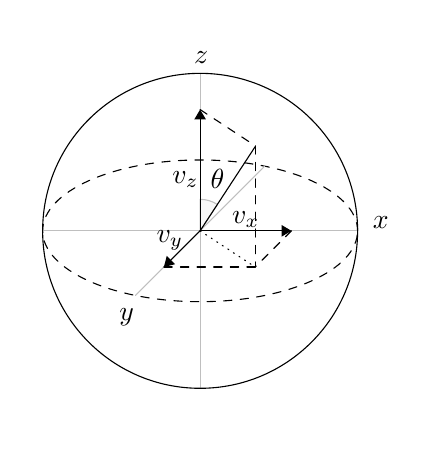
\begin{tikzpicture}[scale = 1.0, line cap=round, line join=round, >=Triangle]
		% equator
		\draw [rotate around={0.:(0.,0.)},dash pattern=on 3pt off 3pt] (0,0) ellipse (2cm and 0.9cm);
		% axis
		\draw [lightgray] (0,-2) -- (0,2);
		\draw [lightgray] (0.82,0.82) -- (-0.82,-0.82);
		\draw [lightgray] (-2,0) -- (2,0);
		% main circle
		\draw(0,0) circle (2cm);
		\clip(-2.19,-2.49) rectangle (2.66,2.58);
		% angle
		\draw [shift={(0,0)}, lightgray, fill, fill opacity=0.1] (0,0) -- (56.7:0.4) arc (56.7:90.:0.4) -- cycle;
		% circles
		% vectors
		\draw (0,0) -- (0.70,1.07);
		\draw [dashed] (0.7,1.08) -- (0.7,-0.46);
		\draw [dashed] (1.16,0) -- (0.7,-0.46);
		\draw [dotted] (0,0) -- (0.7,-0.46);
		\draw [dashed] (0,1.54) -- (0.7,1.08);
		\draw [dashed] (-0.46,-0.46) -- (0.7,-0.46);
		\draw [->] (0,0) -- node[below left=-3] {$v_z$} (0,1.54);
		\draw [->] (0,0) -- node[above=-2.5] {$v_x$} (1.16,0);
		\draw [->] (0,0) -- node[above left=-4] {$v_y$}(-0.46,-0.46);
		% symbols
		\draw (0.01,0.9) node[anchor=north west] {$\theta$};
		\draw (-1.15,-0.86) node[anchor=north west] {$y$};
		\draw (2.07,0.3) node[anchor=north west] {$x$};
		\draw (-0.2,2.4) node[anchor=north west] {$z$};
		
		%\draw (0.4,1.65) node[anchor=north west] {$|\psi\>$};
		% decoration
		\scriptsize
		%\draw [fill] (0,0) circle (1.5pt);
		%\draw [fill] (0.7,1.1) circle (0.5pt);
	\end{tikzpicture} 
	\caption{A direction in space or a pure state on the Bloch sphere.\protect\footnotemark}
\end{figure}
\footnotetext{\label{note1}Figures contributed by Aleksi Winstén}

A direction in space is identified by a normalized vector in a three dimensional space. Though these can be identifies by two angles, the linearity is best expressed in Cartesian components.
\begin{equation}
	\begin{aligned}
		v^x e_x + v^y e_y + v^z e_z &= \cos \varphi \sin \theta e_x + \sin \varphi \sin \theta e_y + \cos \theta e_z \\
		(v^x)^2 + (v^y)^2 + (v^z)^2 &= 1 \\
		&= \cos^2 \varphi \sin^2 \theta + \sin^2 \varphi \sin^2 \theta + \cos^2 \theta \\
		&= ( \cos^2 \varphi + \sin^2 \varphi ) \sin^2 \theta + \cos^2 \theta
	\end{aligned}
\end{equation}
Note how the basis is composed by orthogonal directions in space and that the constraint is quadratic in those components.

\begin{figure}[h]
	\centering
	\begin{minipage}{0.48\textwidth}
		\centering
		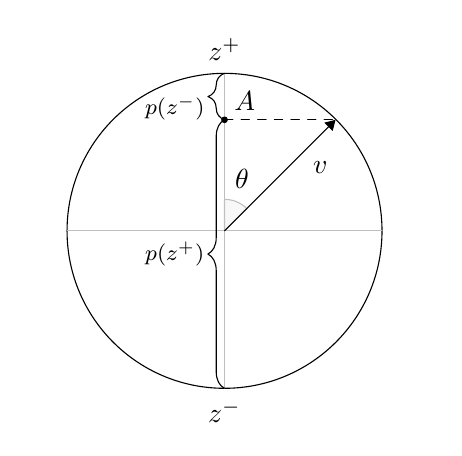
\begin{tikzpicture}[scale = 1.0, line cap=round, line join=round, >=Triangle]
			\clip(-2.5,-2.5) rectangle (2.66,2.58);
			% angle
			\draw [shift={(0,0)}, lightgray, fill, fill opacity=0.1] (0,0) -- (45:0.4) arc (45:90.:0.4) -- cycle;
			% circle
			\draw(0,0) circle (2cm);
			% guides
			\draw [lightgray] (-2,0)-- (2,0);
			\draw [lightgray] (0,-2)-- (0,2);
			% vector
			\draw [->] (0,0) -- (1.41,1.41);
			\draw [dashed] (0,1.41)-- (1.41,1.41);
			% brackets
			\draw[decorate,decoration={brace, amplitude = 6pt, raise = 0pt}] (0,-2) -- (0,1.41) node[midway, xshift = -18pt]{\footnotesize $p(z^+)$};
			\draw[decorate,decoration={brace, amplitude = 6pt, raise = 0pt}] (0,1.41) -- (0,2) node[midway, xshift = -18pt, yshift = -4pt]{\footnotesize $p(z^-)$};
			% symbols
			\draw (0.01,0.9) node[anchor=north west] {$\theta$};
			\draw (0,1.41) node[anchor=south west] {$A$};
			\draw (1,1) node[anchor=north west] {$v$};
			\draw (0,2.3) node[] {$z^+$};
			\draw (0,-2.3) node[] {$z^-$};
			% decoration
			\scriptsize
			\draw [fill] (0,1.41) circle (1pt);
		\end{tikzpicture}
		\par\small States (projective space)
	\end{minipage}
	\begin{minipage}{0.48\textwidth}
		\centering
		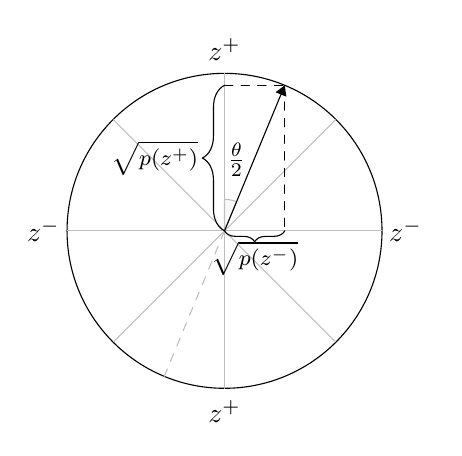
\begin{tikzpicture}[scale = 1.0, line cap=round, line join=round, >=Triangle]
			\clip(-2.5,-2.5) rectangle (2.66,2.58);
			% angle
			\draw [shift={(0,0)}, lightgray, fill, fill opacity=0.1] (0,0) -- (67.5:0.4) arc (67.5:90.:0.4) -- cycle;
			% circle
			\draw(0,0) circle (2cm);
			% guides
			\draw [lightgray] (-2,0)-- (2,0);
			\draw [lightgray] (0,-2)-- (0,2);
			\draw [lightgray] (-1.41,-1.41)-- (1.41,1.41);
			\draw [lightgray] (1.41,-1.41)-- (-1.41,1.41);
			% vector
			\draw [->] (0,0) -- (0.765,1.848);
			\draw [lightgray,dashed] (0,0) -- (-0.765,-1.848);
			\draw [dashed] (0,1.848)-- (0.765,1.848);
			\draw [dashed] (0.765,1.848)-- (0.765,0);
			% brackets
			\draw[decorate,decoration={brace, amplitude = 8pt, raise = 0pt}] (0,0) -- (0,1.848) node[midway, left = 6pt]{\footnotesize $\sqrt{p(z^+)}$};
			\draw[decorate,decoration={brace, amplitude = 4pt, raise = 0pt, mirror}] (0,0) -- (0.765,0) node[midway, xshift = 0pt, yshift = -10pt]{\footnotesize $\sqrt{p(z^-)}$};
			% symbols
			\draw (0.15,0.9) node[] {$\frac{\theta}{2}$};
			% \draw (1,1) node[anchor=north west] {$\mathbf {V}$};
			\draw (0,2.3) node[] {$z^+$};
			\draw (0,-2.3) node[] {$z^+$};
			\draw (-2.3,0) node[] {$z^-$};
			\draw (2.3,0) node[] {$z^-$};
			% decoration
			\scriptsize
		\end{tikzpicture}
		\par\small State vectors
	\end{minipage}
	\caption{On the left, quantum states on the projective space. On the right, quantum state on the vector space.\textsuperscript{\ref{note1}}}
\end{figure}

In quantum mechanics, we are interested in probability of outcomes of a directional measurement. If we fix a direction, two outcomes are possible. For any other state, the probability of outcome must be proportional to the component in that direction. For a measurement along the $z$ direction, the probabilities must be:
\begin{equation}
	\begin{aligned}
		p(z^+) &= \frac{\overline{A z^-}}{\overline{z^+ z^-}} = \frac{1+\cos \theta}{2} = \cos^2 \frac{\theta}{2} \\
		p(z^-) &= \frac{\overline{z^+ A}}{\overline{z^+ z^-}} = \frac{1-\cos \theta}{2} = \sin^2 \frac{\theta}{2} \\
		p(z^+) + p(z^-)&= 1 \\
		&= (v^x)^2 + (v^y)^2 + (v^z)^2 = 1 \\
		&= \frac{1+\cos \theta + 1-\cos \theta}{2} = \cos^2 \frac{\theta}{2} + \sin^2 \frac{\theta}{2}
	\end{aligned}
\end{equation}
Note how the outcomes are a set of opposite direction and the constraint is linear. However, it can be re-expressed as quadratic in terms of the square root of the probability and half the angle. This is what allows us to represent states in a vector space.

For a qubit, spin 1/2, two-state system, states are represented by
\begin{equation}
	\begin{aligned}
		| \psi \> &= \cos \frac{\theta}{2} e^{-\imath \frac{\varphi}{2}} | z^+ \> + \sin \frac{\theta}{2} e^{\imath \frac{\varphi}{2}} | z^+ \> \\
		p(z^+) &= \<\psi | z^+ \> \< z^+ | \psi \> = \cos \frac{\theta}{2} e^{\imath \frac{\varphi}{2}} \cos \frac{\theta}{2} e^{-\imath \frac{\varphi}{2}} = \cos^2 \frac{\theta}{2} \\
	p(z^-) &= \<\psi | z^- \> \< z^- | \psi \> = \sin \frac{\theta}{2} e^{-\imath \frac{\varphi}{2}} \sin \frac{\theta}{2} e^{\imath \frac{\varphi}{2}} = \sin^2 \frac{\theta}{2} \\
		\< \psi | \psi \> &= \cos \frac{\theta}{2} e^{\imath \frac{\varphi}{2}} \cos \frac{\theta}{2} e^{-\imath \frac{\varphi}{2}} + \sin \frac{\theta}{2} e^{-\imath \frac{\varphi}{2}} \sin \frac{\theta}{2} e^{\imath \frac{\varphi}{2}} \\
		&= \cos^2 \frac{\theta}{2} + \sin^2 \frac{\theta}{2} \\
	\end{aligned}
\end{equation}
The norm of the components, and therefore $\theta$, fixes the height of the vertical plane that cuts the sphere, while the phase, and therefore $\varphi$, fixes the angle along the identified circle.

Multiple vectors represent the same state. For example, $\theta + 2\pi$ gives a different vector with negative components, but the same direction in the original space and the same probability. We can visualize the difference easily by restricting ourselves to the $(x,z)$ plane. A direction in physical space corresponds to a line that passes through the origin (i.e. a ray) in the vector space. A line returns to itself after half a turn.


\end{document}